\documentclass[twocolumn]{article}
\usepackage{epigraph}
\usepackage{lettrine}
\usepackage{graphicx}
\usepackage{hyperref}

\setlength{\epigraphwidth}{\textwidth}
%opening
\title{HSBC-AUS Coding Challenge 2019 Write-up}
\author{Sheikh Abdul Raheem Ali \\ Department of Computer Science and Engineering, American University of Sharjah}
\date{}

\begin{document}

\maketitle

\epigraph{To the beautiful dream of computation, and to those it has inspired to seek its secrets with pleasure and admiration.}

\section*{Introduction}

\lettrine[findent=2pt]{\fbox{\textbf{S}}}{ }tatistical techniques are widely used for various applications in finance. \textsl{Logistic Regression} is one of the most common methods used to estimate the Probability of Default (PD) from a historical database of financial performance.

This paper provides an accessible explanation of how Logistic Regression works, a description of how it can be implemented using Python, and a discussion of why a regularized binary logistic model was chosen above more ``sexy'' machine learning algorithms like Support Vector Machines (SVMs), Naive Bayes, Random Forests, and Neural Networks.

In particular, the author hopes that the reader is left with an appreciation for fundamental data science concepts like pre-processing, stability, regression, dimensionality, classification, and optimization.  

\section*{Logistic Regression}

In mathematics, regression can be thought of as finding the best fitting curve given a set of points embedded in some space. The goal in logistic regression is to model the probability of some binary outcome $  P(Y = 1) $ given some input $ X $, although many complex extensions exist.



\begin{figure}[h]
	\centering
	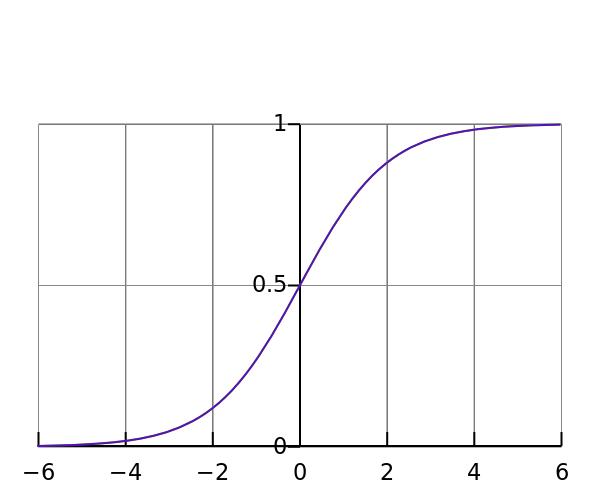
\includegraphics[width=\linewidth]{Logistic-curve.png}
	\caption{The shape of the curve we are trying to fit in logistic regression, known as a sigmoid.}
\end{figure}
 
\section*{Advantages}

\begin{itemize}
	\item \textbf{Speed.} The model training and testing only took a few seconds on my 2.20GHz machine. 
	\item \textbf{Popularity.} Fun fact, MATLAB's financial toolbox's probdefault function uses logistic regression.
	\item \textbf{Interpretability.} A trained model has regression co-efficients that can (using the likelihood-ratio test) help us determine how each variable contributes to the final result.
	\item \textbf{Robustness.} Regularized logistic regression is stable. It can handle erroneous, sparse, unbalanced input without failure. This is especially important because some values are missing in the dataset, and there are only 307 cases of default in the 9968 observations.
	\item \textbf{Accuracy.} Hastie et. al. shows that logistic regression has one of the lowest error rates out of a variety of linear techniques when working with high dimensional data where a few variables account for a large percentage of the variance. 
	\item \textbf{Simplicity.} Scikit-learn's built in logistic regression module already includes a predict\_proba function (and in fact, logistic regression naturally produces the probability of an outcome), so all I had to do was modify its output so that it generated a valid credit score. 
\end{itemize}

\section*{Implementation}

\begin{enumerate}
	\item The training and validation datasets were provided by HSBC in an excel file.
	\item The package openpyxl was used to read this data into python.
	\item Scikit-learn's built in roc\_auc\_score was used to evaluate the performance of different parameter settings during development by partitioning the labeled dataset into training and testing sets which were not mixed. 
	\item The final model was trained using the entire labeled dataset and the default parameters. 
	\item The model's predictions were used to generate credit scores for the validation dataset that were written back into an excel file and saved.
	\item The results and code were submitted to AUS.
\end{enumerate}

\section*{Discussion}

 Logistic Regression is simply better suited to this task and this dataset than most other techniques. Ensemble methods like random forests require thousands of examples of each class to construct accurate models. SVMs are non probabilistic. Naive Bayes is known to be a poor estimator. Neural Networks are more applicable for vision and speech recognition.  Stochastic Gradient Descent requires \textsl{hundreds of thousands} of observations. K-Nearest Neighbors is not suitable for high dimensional data, so one must apply principal component analysis or spectral clustering beforehand. 

\begin{figure}[h]
	\centering
	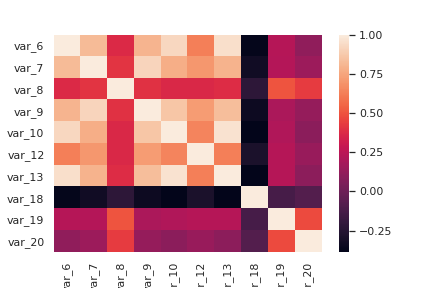
\includegraphics[width=\linewidth]{foo.png}
	\caption{The data is highly correlated}
\end{figure}

In conclusion, while one must strive to push the frontiers of innovation, tried and tested approaches should always be a business's first resort. Understanding the problem and the data first is a necessary prerequisite for designing effective solutions in any field. Every tool has a place on your belt, but sometimes a nail just needs a hammer. 

\section*{References}


\href{https://web.stanford.edu/~hastie/ElemStatLearn/printings/ESLII_print12.pdf}{Friedman, J., Hastie, T., \& Tibshirani, R. (2001). \textsl{The elements of statistical learning} (Vol. 1, No. 10). New York: Springer series in statistics, p. 107.}


\href{https://www.mathworks.com/help/finance/creditscorecard.probdefault.html}{MathWorks, (2018). Financial Toolbox: probdefault (R2018b).}


\href{http://akademik.bahcesehir.edu.tr/~tevfik/courses/cmp5101/cs229-notes1.pdf}{Ng, Andrew (2000). ``CS229 Lecture Notes'' (PDF). \textsl{CS229 Lecture Notes}: pp. 16-19. }

\href{http://www.jmlr.org/papers/v12/pedregosa11a.html}{Pedregosa, F., Varoquaux, G., Gramfort, A., Michel, V., Thirion, B., Grisel, O., ... \& Vanderplas, J. (2011). Scikit-learn: Machine learning in Python. \textsl{Journal of machine learning research}, 12(Oct), 2825-2830.}


\end{document}
